\documentclass[10pt,conference]{IEEEtran}
\IEEEoverridecommandlockouts
% The preceding line is only needed to identify funding in the first footnote. If that is unneeded, please comment it out.
\usepackage{balance}
\usepackage{xspace}
\usepackage{graphicx}
\usepackage[mathscr]{euscript}
\usepackage{listings}
\usepackage{enumitem}
\usepackage{multirow}
\usepackage{amsmath,amssymb}
\usepackage[usenames, dvipsnames]{color}
\usepackage{wrapfig}
\usepackage{cite}
\usepackage{float}
\usepackage[flushleft]{threeparttable}
\usepackage{pifont}
\usepackage{scrextend}
\usepackage{soul}
\usepackage{color} 
\usepackage{fancyvrb}
\usepackage{hyperref}
\usepackage{lettrine}


\def\BibTeX{{\rm B\kern-.05em{\sc i\kern-.025em b}\kern-.08em
    T\kern-.1667em\lower.7ex\hbox{E}\kern-.125emX}}
\begin{document}

\title{Rename Refactorings}

\author{
\IEEEauthorblockN{Soumya Mudiyappa}
\IEEEauthorblockA{\textit{West Chester University}\\fs926226@wcupa.edu}
\and
\IEEEauthorblockN{Swetchha Shukla}
\IEEEauthorblockA{\textit{West Chester University}\\ss928947@wcupa.edu}
\and
\IEEEauthorblockN{Yung-Chen Cheng}
\IEEEauthorblockA{\textit{West Chester University}\\yc917559@wcupa.edu}
}

\maketitle

\section{\textbf{Rename Refactorings}}
\lettrine{R} {ename} Refactoring provides an easy way to change the name of identifiers for code symbols without changing its behavior.
There are five types of Rename Refactoring: 
\begin{enumerate}
	\item Rename Class Declarations 
	\item Rename Method Declarations  
	\item Rename Field Declarations  
	\item Rename Local Variables  
	\item Rename Package Declarations
\end{enumerate}

\section{\textbf{Preconditions of Rename Class Refactoring}}
Rename Class Refactoring (RcR) changes the name of the class and all references to that class to the new name without changing its behavior. There are certain preconditions required for RcR. 
\begin{enumerate}
	\item The target class cannot be duplicate with any existing class within same package after rename.
	\item The target class cannot be duplicate with any imported class from different package after rename.
	\item The target class file name cannot be duplicate with any existing java file name within same package after rename.
\end{enumerate}

\subsection{The target class cannot be duplicate with any existing class within same package after rename.}

When we try to rename a class with any existing class name, the Java compiler produces syntax error \textit{``Please choose another name"}.~\cite{EclipseWebPage} The classes will be conflicted if we rename refactor the target class using the name of an existing class in the same package. So, we can not have duplicate class names in the same package. 

For example, if we want to rename refactor the class name from \textsl{A} to \textsl{B} as in Fig. \ref{fig:afterrr}, then the Java compiler produces an error that B.java already exists as shown in Fig. \ref{fig:renameclassname}.

\begin{figure}[th]
\centering
\begin{minipage}[t]{0.45\linewidth}
\begin{lstlisting}[language=java, basicstyle=\scriptsize\ttfamily,frame=single]
package p;

class A{
}
	
class B{
}

class C{
}
 
\end{lstlisting}
\centering{(a) Before}
\end{minipage}
\hfill
\begin{minipage}[t]{0.45\linewidth}
\begin{lstlisting}[language=java, basicstyle=\scriptsize\ttfamily,frame=single]
package p;

class B{
}	

class B{
}

class C{
}

\end{lstlisting}
\centering{(b) After}
\end{minipage}
\caption{\textbf{Example of RcR from A to B}}
\label{fig:afterrr}
\end{figure}

\begin{figure}[H]
\centerline{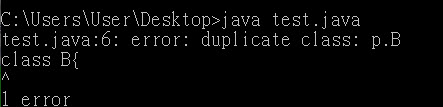
\includegraphics[width=85mm,scale=0.5]{SCN.jpg}}
\caption{\textbf{Compile error for using same class name after RcR}}
\label{fig:renameclassname}
\end{figure}

Also, this precondition is applicable even if the classes are defined in separate java files or any file is empty but are within the same folder. In Fig. \ref{fig:empty}, we try to apply RcR from \emph{A to C} or \emph{B to C} where C.java is an empty file, the compiler produces an error as shown in Fig. \ref{fig:efr}. 

\begin{figure}[th]
\centering
\begin{minipage}[t]{0.45\linewidth}
\begin{lstlisting}[language=java, basicstyle=\scriptsize\ttfamily,frame=single]
A.java

public class A{
}
	
class B{
}


C.java
//empty file
 
\end{lstlisting}
\centering(a) Before
\end{minipage}
\hfill
\begin{minipage}[t]{0.45\linewidth}
\begin{lstlisting}[language=java, basicstyle=\scriptsize\ttfamily,frame=single]
A.java

public class A{
}
	
class C{
}


C.java
//empty file

\end{lstlisting}
\centering(b) After
\end{minipage}
\caption{\textbf{RcR from B to C even if C.java is empty}}
\label{fig:empty}
\end{figure}

\begin{figure}[H]
\centerline{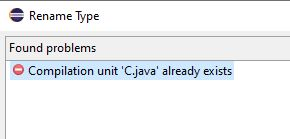
\includegraphics[width=85mm,scale=0.5]{EFE.jpg}}
\caption{\textbf{Compile error for same file name after RcR}}
\label{fig:efr}
\end{figure}


Furthermore, this precondition is also applicable to nested classes. The examples below show that for RcR we can not use the same name either as inner or as outer class for nested classes like Fig. \ref{fig:original}.

\begin{figure}[th]
\centering
\begin{minipage}[t]{0.5\linewidth}
\begin{lstlisting}[language=java, basicstyle=\scriptsize\ttfamily,frame=single]
package p;

public class A{	

  class M{
  }

  class N{
  }
} 
\end{lstlisting}
\end{minipage}
\caption{\textbf{Nested Class before RcR}}
\label{fig:original}
\end{figure}

\textbf{Example 1:} In order to implement RcR for inner class, we should pre-check that we do not use the same name as any of other inner class name. From Fig. \ref{fig:nestedclass1}, when we try to rename refactor the inner class from M to N, the Java compiler produces an error as shown in Fig. \ref{fig:NC1}.

\begin{figure}[th]
\centering
\begin{minipage}[t]{0.5\linewidth}
\begin{lstlisting}[language=java, basicstyle=\scriptsize\ttfamily,frame=single]
package p;

public class A{	
    
  class N{
  }
    
  class N{
  }
} 
\end{lstlisting}
\end{minipage}
\caption{\textbf{Example 1 for Nested Class after RcR from M to N}}
\label{fig:nestedclass1}
\end{figure}

\begin{figure}[H]
\centerline{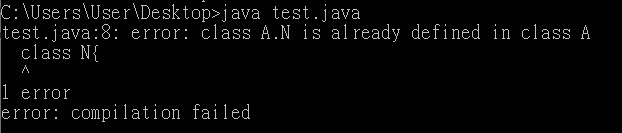
\includegraphics[width=75mm,scale=0.4]{NC1.jpg}}
\caption{\textbf{Compile error for duplicate inner class name after RcR}}
\label{fig:NC1}
\end{figure}

\textbf{Example 2:} In order to implement RcR for outer class, we should pre-check that we do not use the same name as any of the inner class name and vice-versa. From Fig. \ref{fig:nestedclass2}, when we try to use same name for outer class and inner class, the Java compiler produces an error as shown in Fig. \ref{fig:NC2} and Fig. \ref{fig:NC3}.

\begin{figure}[th]
\centering
\begin{minipage}[t]{0.45\linewidth}
\begin{lstlisting}[language=java, basicstyle=\scriptsize\ttfamily,frame=single]
package p;

public class M{	
  
  class M{
  }
	
  class N{
  }
} 
\end{lstlisting}
\centering{(a) After RcR on Outer Class A to M}
\end{minipage}
\hfill
\begin{minipage}[t]{0.45\linewidth}
\begin{lstlisting}[language=java, basicstyle=\scriptsize\ttfamily,frame=single]
package p;

public class A{	
    
  class A{
  }
    
  class N{
  }
} 
\end{lstlisting}
\centering{(b) After RcR on Inner Class N to A}
\end{minipage}
\caption{\textbf{Example 2 of Nested Class after RcR}}
\label{fig:nestedclass2}
\end{figure}

\begin{figure}[H]
\centerline{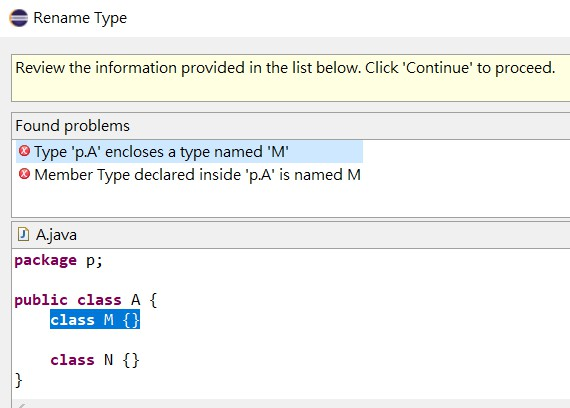
\includegraphics[width=75mm,scale=0.4]{NC2.jpg}}
\caption{\textbf{Compile error for RcR outer class same as inner class name}}
\label{fig:NC2}
\end{figure}

\begin{figure}[H]
\centerline{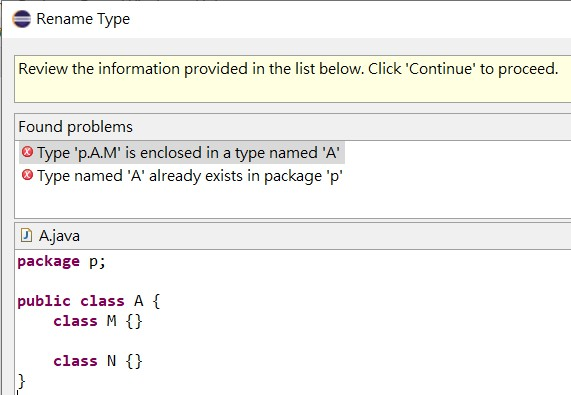
\includegraphics[width=75mm,scale=0.4]{NC3.jpg}}
\caption{\textbf{Compile error for RcR inner class same as outer class name}}
\label{fig:NC3}
\end{figure}

Therefore, checking whether a class with the same name already exists in a package should be the first precondition for RcR. 
   
\label{sec:precon1}
	
\subsection{The target class cannot be duplicate with any imported class from different package after rename.}

If a class is imported from different package, we have to pre-check that the new name of the target class is not duplicate with the imported class after rename refactoring. 

\begin{figure}[th]
\centering
\begin{minipage}[t]{0.4\linewidth}
\begin{lstlisting}[language=java, basicstyle=\scriptsize\ttfamily,frame=single]
package q;
import p.C;

class A{
}

class B{
} 
\end{lstlisting}
\centering(a) Before
\end{minipage}
\hfill
\begin{minipage}[t]{0.4\linewidth}
\begin{lstlisting}[language=java, basicstyle=\scriptsize\ttfamily,frame=single]
package q;
import p.C;

class A{
}

class C{
} 
\end{lstlisting}
\centering(b) After
\end{minipage}
\caption{\textbf{RcR from B to C}}
\label{figure:fig2}
\end{figure}

In Fig. \ref{figure:fig2} (a), we see that class B is not duplicate with class A and we can implement RcR on class B to any other name except `A' as mentioned in section \ref{sec:precon1}. However, in Fig. \ref{figure:fig2} (b), when we try to implement RcR from \emph{B to C}, Java compiler produces an error \textit{``a compilation unit must not import and declare a type with the same name''}~\cite{EclipseWebPage} as shown in Fig. \ref{figure:comperr}. This is because the compiler cannot distinguish between the \emph{imported class C} of package `p' and the \emph{existing class C} of package `q'. 

\begin{figure}[H]
\centerline{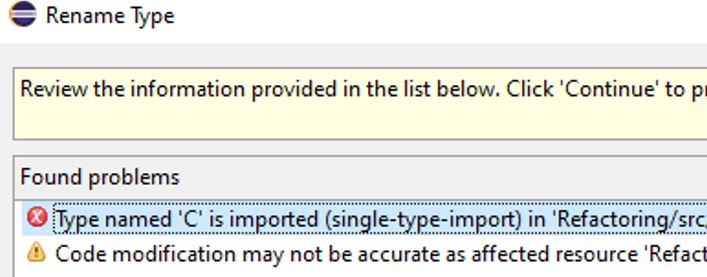
\includegraphics[width=85mm,scale=0.5]{CUE.jpg}}
\caption{\textbf{Compilation Unit Error} }
\label{figure:comperr}
\end{figure}

Therefore, it is essential to pre-check that the target class should not have duplicate name with any of imported class after RcR.
\label{sec:precon2}

\subsection{The target sub-class cannot be duplicate with any imported class into its parent class from another package.}

If we try renaming a subclass with the same name as the class imported into its parent class from another package, compiler produces the error as `a compilation unit must not import and declare a type with the same name'~\cite{EclipseWebPage}. 
To rename a class or subclass for refactoring the code, some of the necessary preconditions have to be checked. This precondition can be explained by the following example.

\begin{figure}[th]
\centering
\begin{minipage}[t]{0.45\linewidth}
\begin{lstlisting}[language=java, basicstyle=\scriptsize\ttfamily,frame=single]	
package q;
import p.C;
class A{	
}
class B extends A{	
}	
\end{lstlisting}
\tiny{(a) Before renaming Subclass B}
\end{minipage}
\hfill
\begin{minipage}[t]{0.45\linewidth}
\begin{lstlisting}[language=java, basicstyle=\scriptsize\ttfamily,frame=single]
package q;
import p.C;
class A{	
}
class C extends A{	
}	
\end{lstlisting}
\tiny{(b) After Renaming Subclass B to C}
\end{minipage}
\caption{Precondition for Renaming Sub-class}
\label{figure:fig7}
\end{figure}

From the above figure \ref{figure:fig7}, We see that if one has imported class C from  package  p to the parent Class A and if we try to rename the sub-class B to C, Compiler produces  the error as given in the figure \ref{figure:fig8} . As mentioned in  section \ref{sec:precon2}, the same precondition also holds good for renaming a sub-class. Before renaming the sub-class, one has to check the precondition that the  target sub-class cannot be duplicate with any imported class into its parent class from another package.

\begin{figure}[htbp]
\centerline{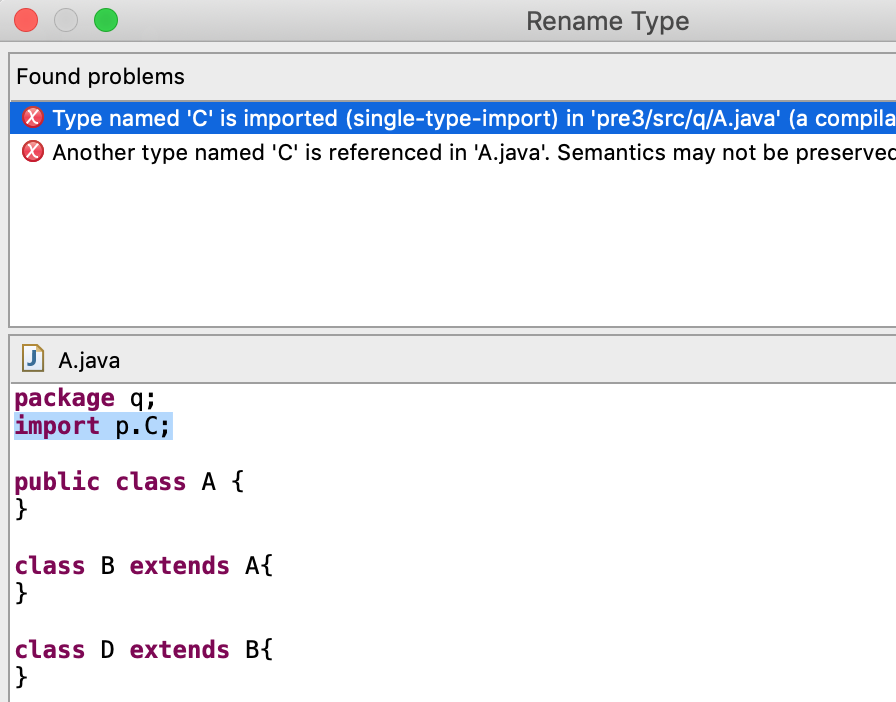
\includegraphics[width=85mm,scale=0.5]{precond3.png}}
\caption{Error produced after renaming the sub-class.}
\label{figure:fig8}
\end{figure}
\label{sec:precon3}

\section{\textbf{Preconditions of Rename Method Refactoring}}

\section{\textbf{Preconditions of Rename Field Refactoring}}

\section{\textbf{Preconditions of Rename Local Variable Refactoring}}

Rename Local Variable Refactoring (RlR) changes the name of the local variable and all references to that variable to the new name without changing its behavior. There are certain preconditions required for RlR.

\subsection{The target name of local variable cannot be duplicate with the name of the input parameter of the method.}

\begin{figure}[th]
\centering
\begin{minipage}[t]{0.45\linewidth}
\begin{lstlisting}[language=java, basicstyle=\scriptsize\ttfamily,frame=single]
public class A {
   int i = 0;
   
   void m1(int num) {
	int x = 7;
    }
}
\end{lstlisting}
\centering(a) Before
\end{minipage}
\hfill
\begin{minipage}[t]{0.45\linewidth}
\begin{lstlisting}[language=java, basicstyle=\scriptsize\ttfamily,frame=single]
public class A {
   int i = 0;
   
   void m1(int num) {
	int num = 7;
    }
}
\end{lstlisting}
\centering(b) After
\end{minipage}
\caption{\textbf{RlR from x to num}}
\label{figure:precond5_1}
\end{figure}

For example, from Fig. \ref{figure:precond5_1}, when we apply RlR for local variable `x' to `num' , the java compiler produces the error as ``variable num is already defined in method m1(int)'' and this creates a conflict as duplicate local variable.

Therefore, it is essential to pre-check that the target name of local variable should not have duplicate name with the input parameter of the method after RlR.



\section{\textbf{Preconditions of Rename Package Refactoring}}

%\bibliographystyle{IEEEtran}
%\bibliography{ref}

\end{document}
